% -----------------------------------------------------------------------------
% Metodologia
% -----------------------------------------------------------------------------

\chapter{Metodologia}
\label{chap:metodologia}

O desenvolvimento do presente trabalho parte da premissa de que designers e desenvolvedores não tem uma linguagem comum durante a execução de suas atividades, produzindo artefatos isoladamente uns dos outros. Por conta disso, problemas como inconsistência no produto, baixa velocidade de desenvolvimento de novas interfaces de usuário e dificuldade em se dar manutenção em interfaces já existente, são alguns dos fatores que comprometem a capacidade de escalabilidade dos produtos de empresas de tecnologia.

Para entender se a proposta de metodologia de um \textit{design system} é eficiente para resolver tais problemas no processo de design e desenvolvimento \textit{frontend} das organizações, o autor deste trabalho se baseou na Dito, empresa de tecnologia sediada na cidade de Belo Horizonte - Minas Gerais, para um experimento de sua proposta. Com 11 anos de história, a empresa vem passando por um processo de crescimento bastante acelerado. Por conta disso, muitos dos sintomas que impedem a escalabilidade do seu produto já são perceptíveis internamente na organização. 

O experimento realizado tem como objetivo construir um protótipo de um \textit{design system}, validando se os benefícios indicados pela teória da metodologia realmente se manifestam na prática. Sabendo que a construção de um \textit{design system} é uma tarefa muito complexa, o autor optou por incluir somente o artefato de biblioteca de componentes no protótipo. Como temática para o projeto, foi proposta a construção de um sistema de gestão de funcionários da empresa, intitulado \textit{DitoFeras}.

A metodologia adotada no desenvolvimento deste trabalho é dividida em cinco grandes estágios, ilustrados através da \autoref{fig:metodology}.

\begin{figure}
	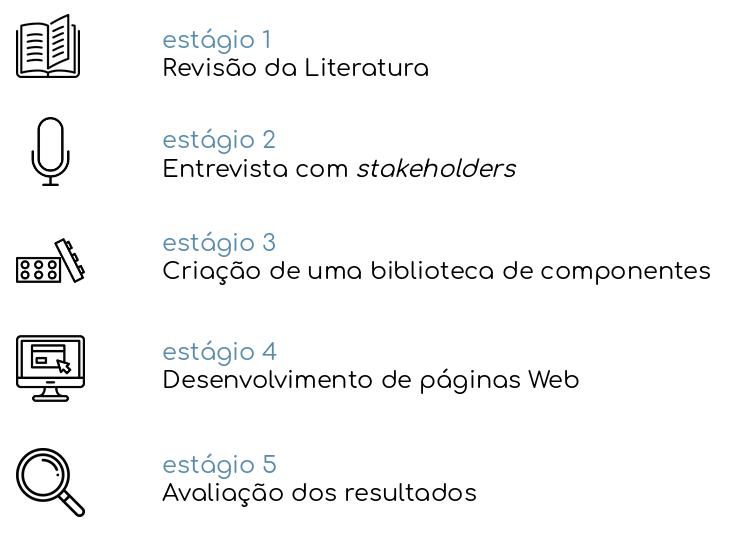
\includegraphics[width=\linewidth]{./04-figuras/04_metodologia/metodologia.png}
  \caption{Esquema da metodologia}
  \fonte{Próprio autor}
  \label{fig:metodology}
\end{figure}

O estágio inicial da metodologia tinha como objetivo realizar uma revisão de trabalhos e estudos relacionados a \textit{design systems}, tanto no âmbito acadêmico quanto no industrial. As informações adquiridas nesse estágio foram apresentadas mais detalhadamente nos capítulos \ref{chap:fundamentacaoTeorica} e \ref{chap:trabRelac} deste trabalho e serviram como base de conhecimento para os estágios seguintes.

No segundo estágio, foram realizadas entrevistas com os principais \textit{stakeholders} do projeto: designers e desenvolvedores. A ideia das entrevistas é validar se os colaboradores se sentem incomodados com a maneira que os processos de design e desenvolvimento da empresa são adotados atualmente. Em caso positivo, seguiria-se para o estágio seguinte da metodologia.

No estágio 3, caso seja comprovada sua necessidade pelo estágio anterior, daria-se início ao desenvolvimento de uma biblioteca de componentes simples. Seguindo a ideia da Ryte \cite{ryteDesignSystem} para a criação do seu \textit{design system}, a versão de protótipo da biblioteca de componentes da Dito seria baseada em dois artefatos: um guia de design, construído utilizando a ferramenta Figma \footnote{O Figma é uma ferramenta de design gráfico voltada para prototipação de interfaces de usuário. É um dos concorrentes do Sketch e está disponibilizado em <https://www.figma.com/>.}, e um repositório Git com a implementação dos componentes. Com os componentes construídos, seguiria-se para o estágio 4 da metodologia.

O quarto estágio seria aquele que, tomando como base os componentes criados no estágio anterior, construiria algumas páginas Web propostas para o projeto \textit{DitoFeras}. Esperava-se que, nessa fase, a velocidade de desenvolvimento das páginas fosse mais rápida do que aquela habitual. Por fim, o último estágio seria aquele que definiria e mediria as métricas de performance do experimento, comprovando ou não a eficácia de um \textit{design system}.

No capítulo seguinte será apresentado detalhadamente os resultados obtidos no segundo estágio da metodologia deste projeto: entrevistas com \textit{stakeholders}.
